\documentclass{article}

% Language setting
% Replace `english' with e.g. `spanish' to change the document language

\usepackage[english]{babel}

% Set page size and margins
% Replace `letterpaper' with `a4paper' for UK/EU standard size

\usepackage[letterpaper,top=2cm,bottom=2cm,left=3cm,right=3cm,marginparwidth=1.75cm]{geometry}

% Useful packages
\usepackage{amsmath}
\usepackage{graphicx}
\usepackage[colorlinks=true, allcolors=blue]{hyperref}
\usepackage{authblk}
\usepackage{amsfonts}

\title{\huge \textbf{Resurrected Cat Paradox: Challenging the Von Neumann-Wigner Interpretation of Quantum Mechanics}}

\author{\Large Riddhiman Bhattacharya}

\date{July 9, 2023}

\begin{document}
\maketitle
\Large 
\begin{abstract}
\Large

The quantum measurement problem focuses on how the collapse of the wave function occurs[1]. According to the widely known \textbf{Copenhagen Interpretation}[14], wave function collapse happens when a particle is measured. However, a sub-interpretation called the Von Neumann-Wigner Interpretation [2] suggests that consciousness plays a role in wave function collapse. This idea stems from Wigner's friend's thought experiment[3] and raises profound philosophical questions about the impact of consciousness on physical events. Although the Von Neumann-Wigner Interpretation is largely dismissed today, some physicists still consider it valid.

A novel paradox challenging the Von Neumann-Wigner Interpretation[8] is called the Resurrected Cat Paradox, which utilizes the Delayed Choice Experiment and the concept of consciousness causing wave function collapse, serves as a counterargument to the Von Neumann-Wigner Interpretation.

There are additional objections to the Von Neumann-Wigner Interpretation. Even Eugene Wigner, one of its proponents, distanced himself from the interpretation over time. Physicists like Roger Penrose have also pointed out that the evolution of conscious life relies on the collapse of the wave function, making it impossible for consciousness to be the sole cause of collapse.[4,6,7]

\end{abstract}


\section{\Large Fundamentals of Quantum Mechanics}

\subsubsection{\Large \textbf{Wavefunction}}
In classical mechanics we can predict the position $x(t)$ and momentum $p(x,t)$ of a particle as a function of time(t) when given the initial conditions and the forces acting on the particle. However, in quantum mechanics that is not the case. Rather we attempt to find the wave function  $\psi(x,t)$ of the particle.[5,12]

To calculate this wave function we need to solve the Schr\"{o}dinger equation:
\begin{equation}
i\hbar \frac{\partial \Psi}{\partial t} = -\frac{\hbar^2}{2m}
\frac{\partial^2 \Psi}{\partial x^2} + V \Psi
\label{eq:1}
\end{equation}

This seemingly arbitrary function has an important physical significance, given by Born's statistical interpretation: $\int_a^b |\Psi(x,t)|^2 dx$ signifies the probability of finding a particle between \textit{a} and \textit{b} at a time \textit{t} given its wave function


This means that quantum mechanics is indeterminate, that is, you cannot predict the outcome of any experiment, but you can gain statistical information about all the possible outcomes. However, we can say with certainty that the particle has to be somewhere in space and time. Therefore, we can normalise the wave function (provided it is square integrable).

\begin{equation}
\int\limits_{-\infty}^\infty |\Psi(x,t)|^2 dx = 1
\label{eq:2}
\end{equation}

This is useful for determining the magnitude of the complex multiplicative factor $A$ (note that we cannot determine the phase of $A$ by normalization), as if 

$\psi(\mathbf{x},\mathbf{t})$ is a solution to \eqref{eq:1}, so is $A\cdot\psi(\mathbf{x},\mathbf{t})$. 


%\begin{multline*}
 % \small \displaystyle f:[a,b]\to \mathbb %{C} {\text{ square integrable on %}}[a,b]\quad \iff \quad\\
  %\int _{a}^{b}|f(x)|^{2}\,\mathrm {d} %x<\infty 
%\label{eq:4}  
%\end{multline*}




\begin{align}
f:[a,b] &\to \mathbb{C} \text{ square integrable on } [a,b] \nonumber \\
\iff \quad &\int_{a}^{b} |f(x)|^{2} \, dx < \infty
\label{eq:3}
\end{align}



An important consequence of the Schrödinger equation is that if a wave function is normalized at any time, the normalization remains preserved[5].  If the normalization hadn't been preserved, then all wave functions would become non-normalizable (not physical states) and the whole theory would collapse as the Born's interpretation would be deemed incompatible with the Schr\"{o}dinger's equation.


\subsubsection{\Large \textbf{What happens when you make a measurement?}}

Let us assume an arbitrary wave function of a particle \ref{fig:Before measurement}, with probabilities of being at different points.


%ADD MORE

\begin{figure}
\centering
     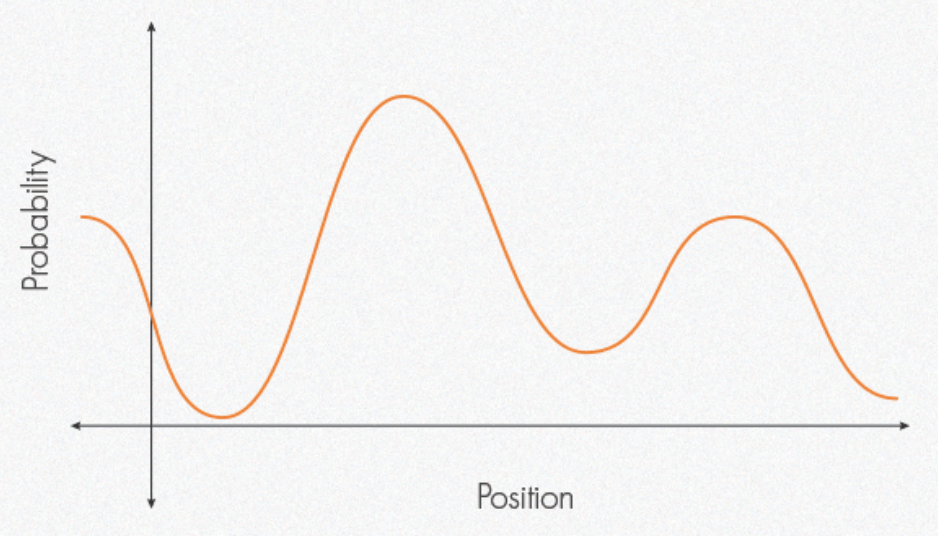
\includegraphics[width=7.5cm,height=7.5cm,keepaspectratio]{Wavefunction before measurement.png}
      \caption{An arbitrary wave function with different probabilities of finding the particle at different points}
       \label{fig:Before measurement}
\end{figure}



The figure in \ref{fig:collapse} represents the Dirac delta function
\begin{equation}
    \delta (x)={\begin{cases}+\infty ,&x=0\\0,&x\neq 0\end{cases}}
    \label{eq:4}\\
    \ \text{Where:} \int _{-\infty }^{\infty }\delta (x)\,dx=1.
\end{equation}

\begin{figure}
\centering
     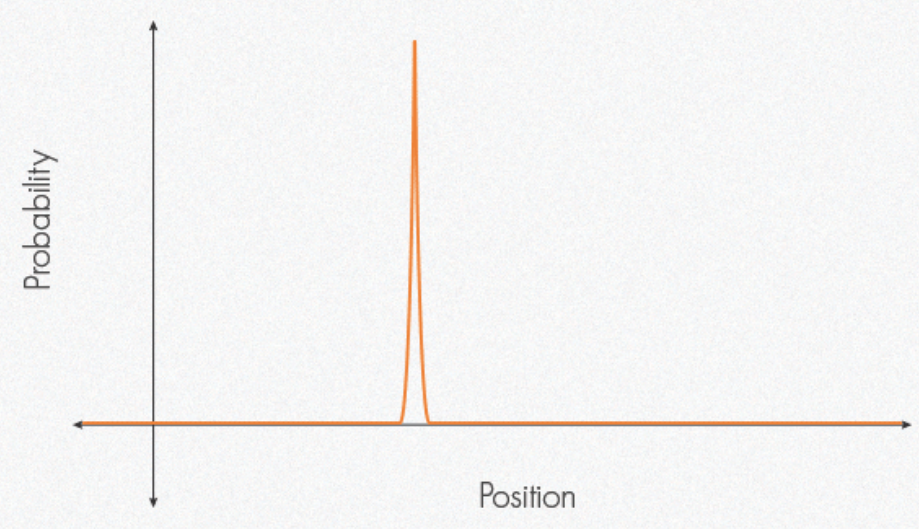
\includegraphics[width=7.5cm,height=7.5cm,keepaspectratio]{Wavefunction after collapse.png}
      \caption{The collapse of the wave function into a delta function when the particle was found at B }
       \label{fig:collapse}
\end{figure}




After the measurement, the wave function instantly spreads out, while obeying the Schr\"{o}dinger equation but with different initial conditions, so the wave function gets modified.

Now, the question arises, when we measured the particle to be at B at some time $t_0$ where is B \textbf{just before} the measurement?

There are three different positions scientists take on this question:
\begin{itemize}
\item \textbf{The realist position}: The realist believes that the particle was at C and quantum mechanics could not predict it, making it an ”incomplete theory” that needs a hidden variable along with the wave function for it to be rendered complete. They believed that nothing is indeterminate and that indeterminacy is just a reflection of our ignorance. 
\item \textbf{The orthodox position}: The particle was not anywhere. You only know where the particle is when you make a measurement, otherwise, its position is indeterminate, and it can be anywhere. We compel the particle to attain a definite position by measuring it. 
\item \textbf{The agnostic position}: The agonist believes that the in-determinacy problem is indeterminable. Because you must make a measurement to know the state of a system, you cannot know the state of a system between measurements. 
\end{itemize}
Interestingly Albert Einstein was a realist, as he believed quantum mechanics defied causality.

All these positions were popular among scientists until Bell's theorem was postulated.


This "\textbf{indeterminacy}" of Quantum mechanics leads to a fundamental quantum mechanical principle.


\section{\Large \textbf{Von Neumann–Wigner Interpretation}}

The \textbf{Von Neumann-Wigner Interpretation} [2,8] is a variant of the \textbf{Copenhagen Interpretation} was developed by \textbf{John von Neumann} and \textbf{Eugene Wigner} and proposes a unique perspective on the collapse of the wave function.

According to the Von Neumann-Wigner Interpretation, \textbf{wave function collapse occurs when a conscious observer interacts with a quantum system.} In this view, the act of measurement is not just a physical process but is also intimately tied to consciousness. The collapse of the wave function happens as a result of the interaction between the measured system and the mind of the observer.

In this interpretation, the role of consciousness is central to the collapse process. It suggests that the observer's consciousness is responsible for determining the outcome of a measurement. The collapse is not seen as an objective, external event but rather as a subjective experience tied to the observer's consciousness.

The Von Neumann-Wigner Interpretation also introduces the idea of the \textbf{mind being the only measurement apparatus}. According to this view, the mind plays a unique role in the collapse of the wave function and is distinct from any physical measurement apparatus used in experiments.

.

\section{\Large \textbf{Double Slit Experiment}}

The Double-Slit Experiment was first conducted by \textbf{Thomas Young} in 1801 as a demonstration of the wave-like behavior of light. Young's setup involved sending light through two narrow slits and observing the pattern formed on a screen placed behind the slits. Surprisingly, an interference pattern emerged on the screen, which is characteristic of waves interacting with each other.

This experiment provided evidence that light behaves not only as particles but also as waves. The interference pattern indicated that light waves passing through the two slits were interfering with each other, resulting in areas of constructive and destructive interference.

\begin{figure}[h]
\centering
     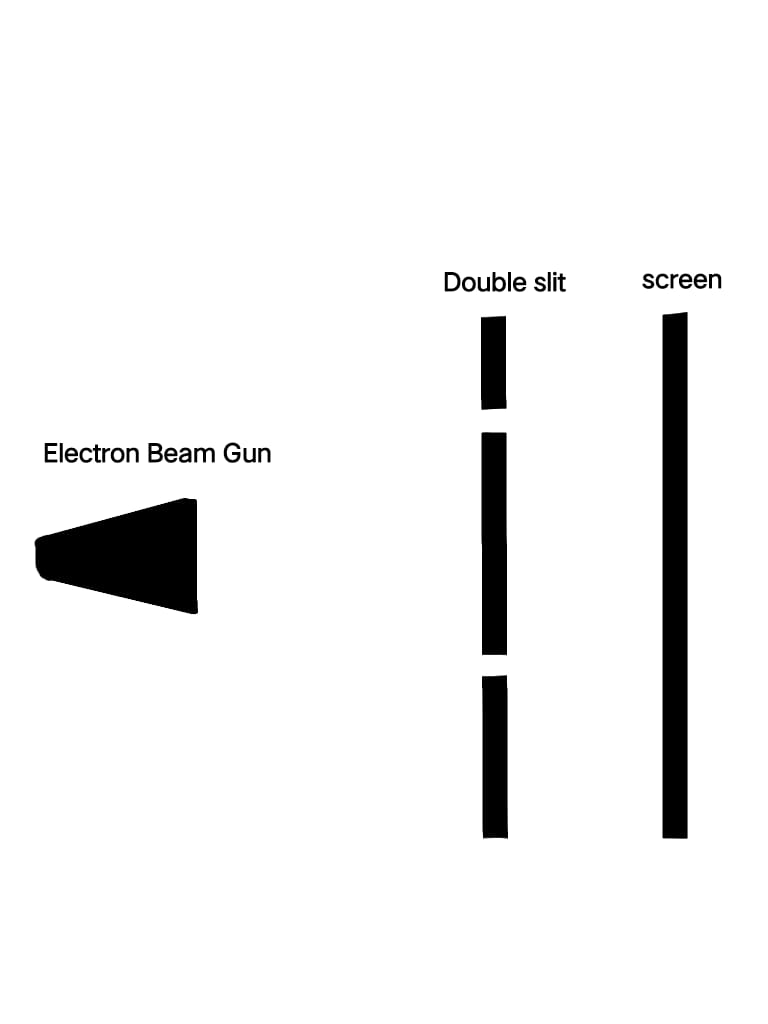
\includegraphics[width=7.5cm,height=7.5cm]{Double Slit.jpeg}
      \caption{\textbf{Double Slit Experiment}}
       \label{fig:DSE}
\end{figure}

In the modern Double-Slit Experiment,[9] electrons are fired towards a screen through two slits. Initially, one would expect the electrons to behave like particles and create a clumped pattern on the screen. However, to the surprise of physicists, the electrons instead generate an interference pattern, indicating wave-like behavior.

Initially, it was thought that the electrons were interfering with each other. However, even when the electrons were shot one by one, the interference pattern persisted. This revealed that the electrons were not interfering with other electrons but with themselves. The electrons exhibited wave-like behavior and passed through both slits simultaneously.

It is important to note that the electrons in this experiment are not particles or waves prior to measurement.[10] Instead, they exist in a superposition state, the wave function form. A
simple Double-Slit Experiment setup is given in \ref{fig:DSE}.
Since the electrons are in a superposition of two states, the
state of electrons that have been shot can be represented



\begin{equation}
    |\Psi\rangle=\frac{1}{\sqrt{2}}|right slit\rangle+ \frac{1}{\sqrt{2}}|left slit\rangle
\end{equation}



\subsection{\Large \textbf{Observer Effects in Double Slit Experiment}}

The setup for the Double-Slit Experiment with observer effects is given in \ref{Setup for Observer Effects }

When a measuring device is placed before the slits in the Double-Slit Experiment to gather information about which slit each electron is passing through, something interesting happens. The interference pattern that was previously observed disappears, and instead, a clumped pattern emerges on the screen. This indicates that the electrons now exhibit particle-like behavior when their paths are measured.


\begin{figure}[h]
    \centering
    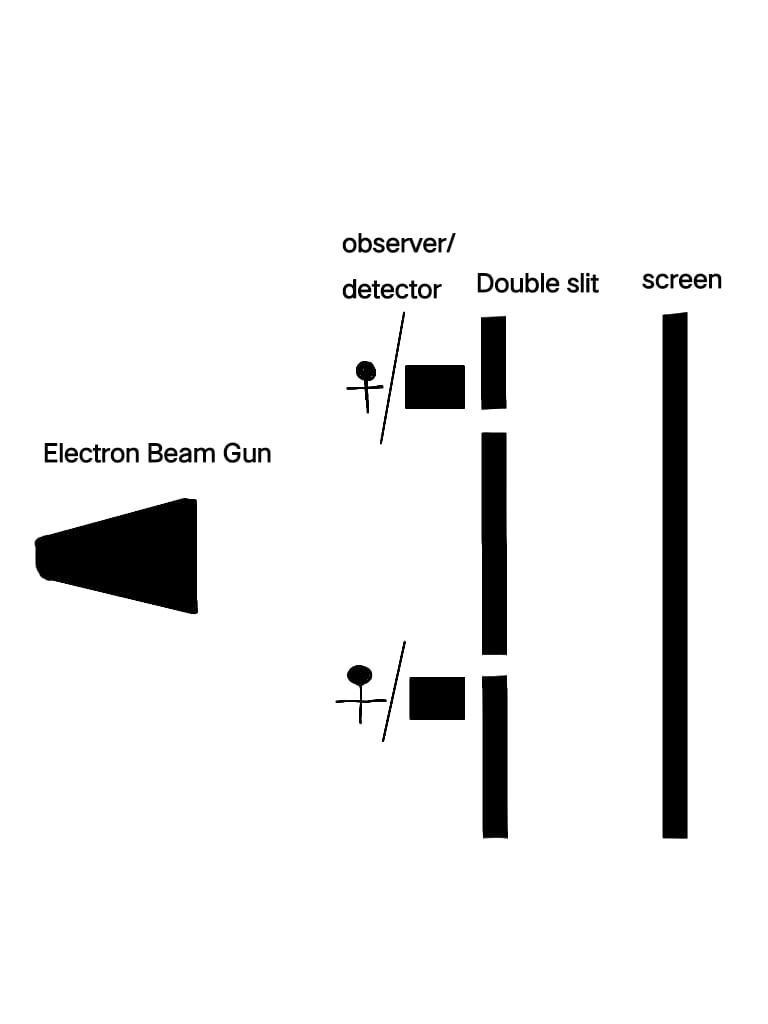
\includegraphics[width=5cm,height=7cm,keepaspectratio]{Observer Effects in Double Slit Experiment.jpeg}
    \caption{\textbf{Setup of Double Slit Experiment taking Observer Effects into account}}
    \label{Setup for Observer Effects }
\end{figure}

The presence of the measuring device and the acquisition of "which-path" information disrupts the wave-like behavior of the electrons. The act of measurement causes the wave function, which describes the probabilistic nature of the electron's position, to collapse. As a result, the electrons behave as particles with definite paths rather than exhibiting wave-like interference.[11]


Since measurement has been made and the wave functions
of the electrons have collapsed, the state of electrons can be
represented as:

\begin{equation}
    |\Psi\rangle=\frac{1}{1}|right slit\rangle+ \frac{0}{1}|left slit\rangle
\end{equation}

\begin{equation}
    |\Psi\rangle=\frac{0}{1}|right slit\rangle+ \frac{1}{1}|left slit\rangle
\end{equation}






\section{\Large \textbf{Delayed Choice experiment}}

The Delayed Choice Experiment \ref{Setup for Delayed Choice Experiment}, proposed by \textbf{John Wheeler}, is similar to the Double-Slit Experiment where the detectors are placed behind the slits, and measurements are made after the electrons pass through. 



\begin{figure}[h]
    \centering 
    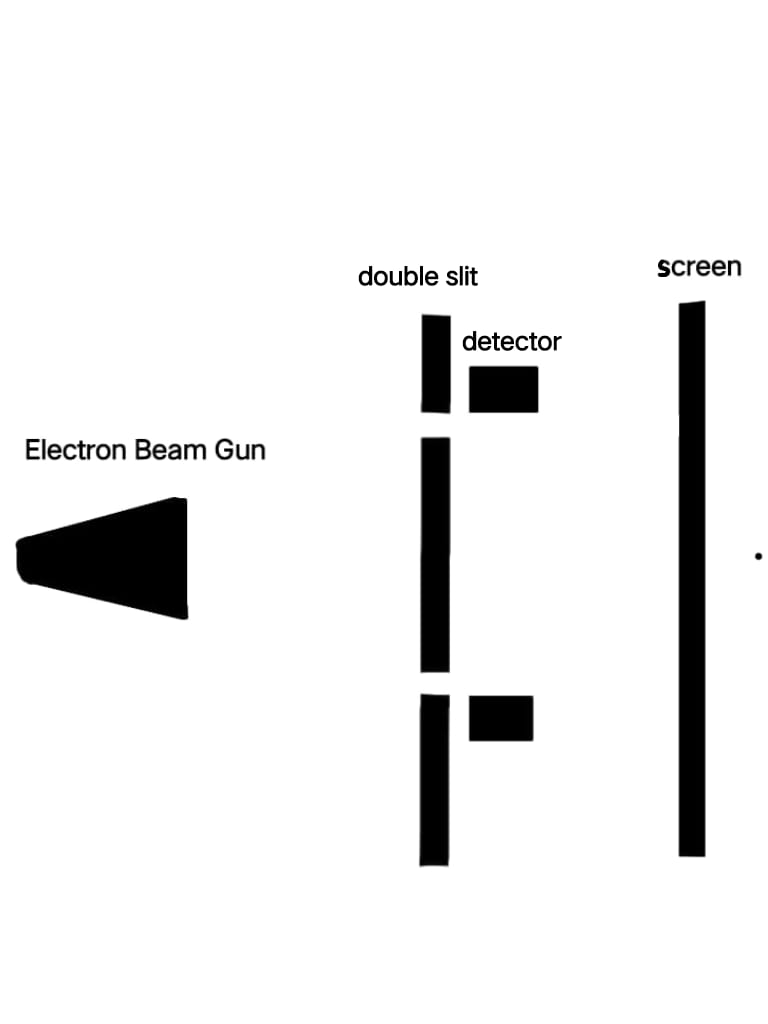
\includegraphics[width=10cm,height=7cm,keepaspectratio]{DCE.jpeg}
    \caption{\textbf{Setup for Delayed Choice Experiment}}
    \label{Setup for Delayed Choice Experiment}
\end{figure}

Surprisingly, even without measuring before the slits, a clumped pattern appears on the screen. This suggests that the electrons behave as wave functions, passing through both slits, but collapsing into a definite path after passing the slits. The experiment's outcome implies that the unobserved past can be altered.[13]



\section{\Large \textbf{The Resurrected Cat Paradox(RCP)}}

The results of the Delayed Choice experiment and the Von
Neumann-Wigner's Interpretations contradict each other. This
contradiction is presented as a paradox \textbf{The Resurrected Cat Paradox (RCP)}. The Setup for RCP is given in Figure \ref{Setup for Resurrected Cat Paradox}

If we assume that the cat is not conscious, we can consider a thought experiment based on the Von Neumann-Wigner Interpretation. In this scenario:

\begin{enumerate}
    \item When the electrons are shot without any observers making observations, the cat dies, since the electron goes through both slits simultaneously. According to the interpretation, the wave function is not collapsed without conscious awareness of the result.


\begin{figure}[h]
    \centering 
    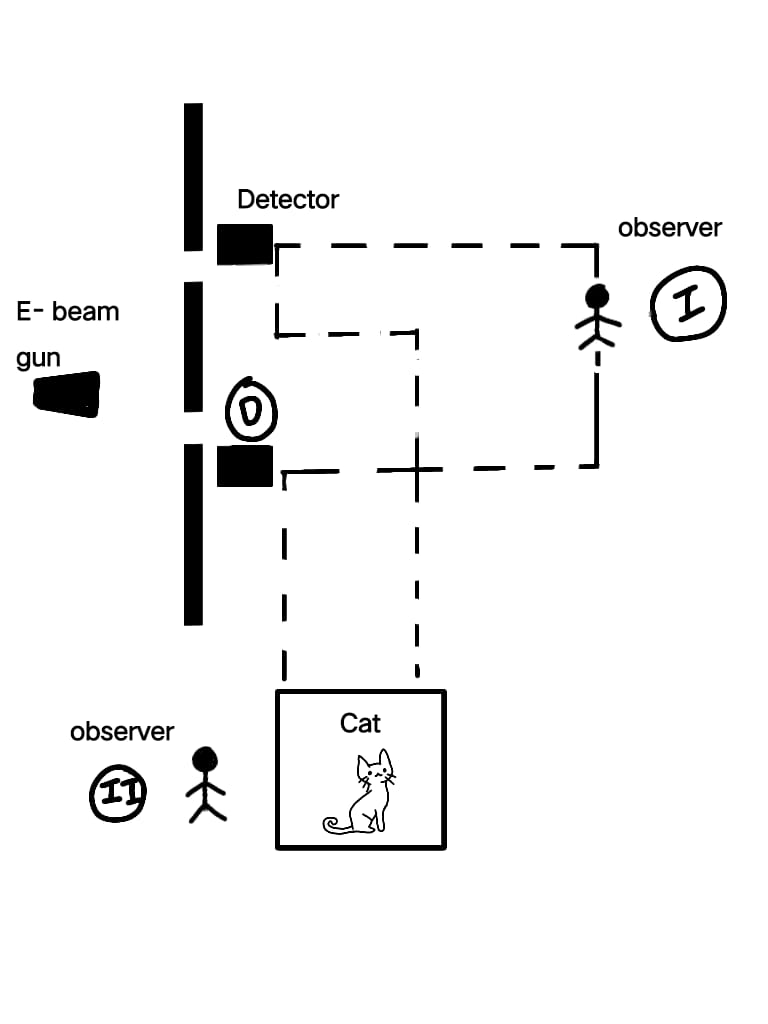
\includegraphics[width=10cm,height=7cm,keepaspectratio]{Resurrected Cat Paradox.jpeg}
    \caption{\textbf{Setup for Resurrected Cat Paradox}}
    \label{Setup for Resurrected Cat Paradox}
\end{figure}



\item  After shooting the electrons and causing the cat's demise, if observer I makes an observation, something intriguing would occur. The interpretation suggests that the observation of observer I could potentially change the unobserved past, specifically the state of the electrons when they passed through the slits. This situation resembles the Delayed Choice Experiment. So, if the past is changed, then the cat's state should also change.


\begin{figure}[h]
\centering
     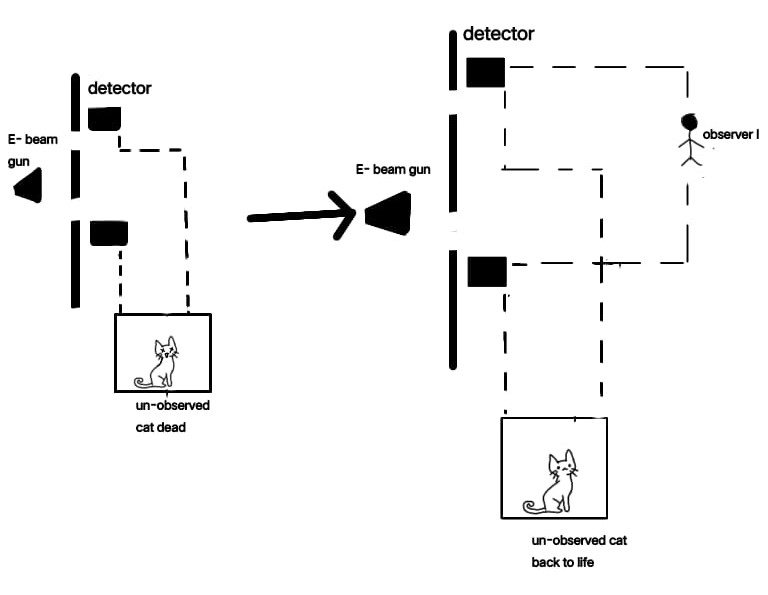
\includegraphics[width=10cm,height=8cm,keepaspectratio]{CASE-1,RCP.jpeg}
      \caption{\textbf{Discussion of RCP-I}}
       \label{}
\end{figure}

\item If, after shooting the electrons and presumably killing the cat, observer II opens the box, they will find the cat dead. However, this particular observation will not cause the collapse of the wave function. This is because finding the dead cat does not provide the observer with any "which path information" about the electrons. As a result, the wave function remains unchanged.

\item Now, let's consider a situation where the electrons have been shot, the cat has been killed, and observer II has observed the dead cat. If observer I makes an additional observation at this point, the interpretation suggests that the cat's state can be changed again. This would alter the previously observed past and bring the cat, which was initially observed as dead, back to life.

\begin{figure}[h]
\centering
     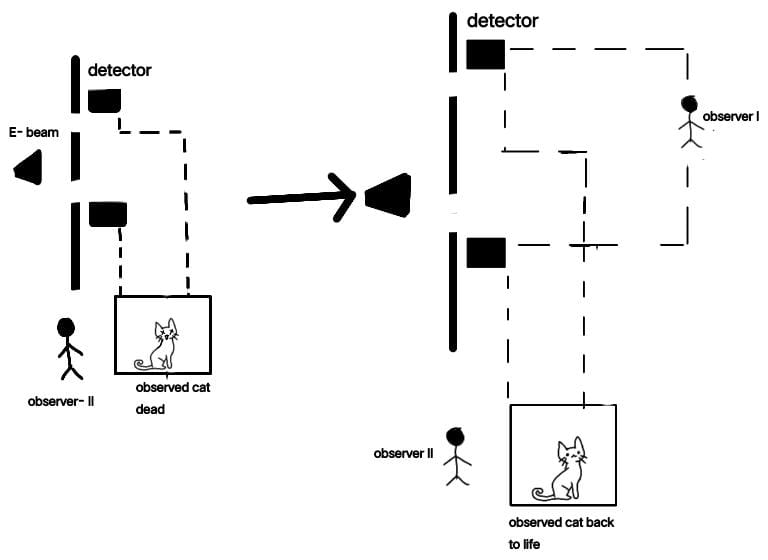
\includegraphics[width=10cm,height=8cm,keepaspectratio]{Case-2, RCP.jpeg}
      \caption{\textbf{Discussion of RCP-II}}
       \label{fig:Wavefn}
\end{figure}
\end{enumerate}

If we consider the scenario where observer II has already observed the dead cat in the box, and then observer I makes their observation, a paradox emerges. If we assume that both observations are valid, we would end up with two contradictory outcomes—one where the cat is dead and one where the cat is alive. This contradicts the fundamental laws of physics.
On the other hand, if we suggest that observer I's observation cannot alter the past, it conflicts with the premise of the experiment itself. The experiment assumes that the past can be changed based on subsequent observations.
RCP challenges the \textbf{Von Neumann-Wigner Interpretation}. According to this interpretation, observer I's observation would have the power to change the past, allowing the cat to come back to life. However, the paradox reveals that such a scenario is not feasible.

Therefore, based on the logical inconsistencies presented by the paradox, we can conclude that the Von Neumann-Wigner Interpretation, which relies on consciousness causing wave function collapse, is incorrect. The experiment's underlying assumptions—that the observable past can be altered and that a cat can be revived after death—cannot hold true.

It's important to note that the experiment itself is not flawed, but rather it exposes the flaws in the Von Neumann-Wigner Interpretation. This realization calls for alternative interpretations of quantum mechanics that can provide more coherent explanations without relying on consciousness as the driving force behind wave function collapse.




\section{\Large \textbf{Acknowledgment}}

I extend my heartfelt gratitude to Ananya Mondal for her tremendous commitment and careful work in drawing all the diagrams used in the paper. The diagrams are an integral part of the paper that significantly improved the readability and comprehension of our work. She spent a lot of time refining them, and I'm very appreciative of that.





\end{document}